\documentclass{tufte-handout}
\usepackage{tikz}
\usepackage{tikz-3dplot}
\usepackage{mathtools}
\usepackage{pgfplots}
\def\salta{\vspace{2cm}}

\usetikzlibrary{shapes,arrows,matrix,fit,positioning,decorations.pathreplacing,3d,calc}
% Diagrams styles
\tikzstyle{block} = [draw=black, rectangle, minimum height=2.5em, minimum width=2em]
\tikzstyle{sum} = [draw=black, circle]
\tikzstyle{gain} = [draw=black, regular polygon, regular polygon sides=3, regular polygon rotate=90, minimum height=2.5em, minimum width=2em]
\tikzstyle{input} = [coordinate]
\tikzstyle{output} = [coordinate]
\tikzstyle{pinstyle} = [pin edge={to-,thin,black}]


\newcommand{\fromworkspace}[3]{%
	\node [block, draw=white,#3, minimum height=1.5em] (#1) {#2};%
	\coordinate [at=(#1.east), xshift=5] (#1_out);%
	\draw (#1.north west) -- (#1.north east) -- (#1_out) -- (#1.south east) -- (#1.south west) -- cycle;%
}
\newcommand{\toworkspace}[3]{%
	\node [block, draw=white,#3] (#1) {#2};%
	\coordinate [at=(#1.west), xshift=-5] (#1_in);%
	\draw (#1.north west) -- (#1.north east) --  (#1.south east) -- (#1.south west) -- (#1_in) -- cycle;%
}
\newcommand{\inputpin}[3]{%
	\node [circle, draw, text width=0.5cm,align=center,#3] (#1) {#2};%
	\coordinate [at=(#1.center), xshift=0.75cm] (#1_out);%
	\draw (#1.north east) -- (#1_out) -- (#1.south east);%
}
\newcommand{\outputpin}[3]{%
	\node [circle, draw, text width=0.5cm,align=center,#3] (#1) {#2};%
	\coordinate [at=(#1.center), xshift=-0.75cm] (#1_in);%
	\draw (#1.north west) -- (#1_in) -- (#1.south west);%
}

\newcommand{\riferimento}{%
\draw[tdplot_rotated_coords,color=blue,thick,->] (0,0,0) -- (2,0,0) node[anchor=east]{$x’$};%
\draw[tdplot_rotated_coords,color=blue,thick,->] (0,0,0) -- (0,2,0) node[anchor=north]{$y’$};%
\draw[tdplot_rotated_coords,color=blue,thick,->] (0,0,0) -- (0,0,2) node[anchor=west]{$z’$};%
}
\newcommand{\ground}{%
\draw[color=red,thick,->] (0,0,0) -- (2,0,0) node[anchor=east]{$x’$};%
\draw[color=red,thick,->] (0,0,0) -- (0,2,0) node[anchor=north]{$y’$};%
\draw[color=red,thick,->] (0,0,0) -- (0,0,2) node[anchor=west]{$z’$};%
}

\begin{document}
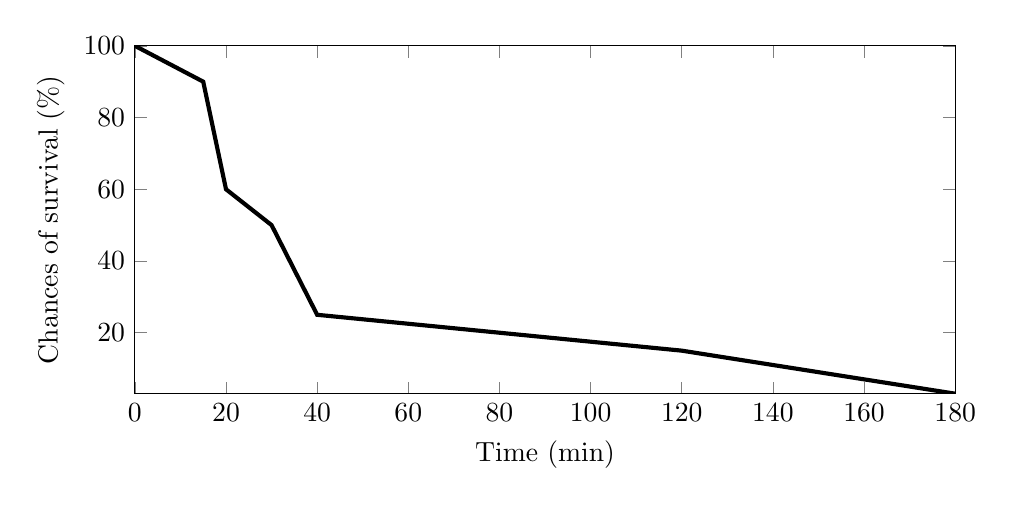
\begin{tikzpicture}
\begin{axis} [xlabel={Time (min)}, ylabel={Chances of survival (\%)},
 enlargelimits=false, width=12cm,height=6cm]

	\addplot [mark=none,line width=1.5] coordinates {
		(0,100)
		(15,90)
		(20,60)
		(30,50)
		(40,25)
		(120,15)
		(180,3)
	};
\end{axis}

\end{tikzpicture}


%
%\begin{tikzpicture}
%
%\begin{semilogxaxis}[xlabel={Frequency (Hz)}, ylabel={Magnitude (dB)},
%xmin=10^3, xmax=10^8, ymin=-150, ymax=60, 
%height=5cm, width=6cm, 
%grid=both, grid style={color=gray!40, dotted}, 
%tick label style={font=\scriptsize},
%xminorticks=true, 
%scaled ticks=true,
%log basis x=10,
%enlargelimits=false]
%
%	\addplot[mark=none,line width=1.5] file {filter1.txt};
%\end{semilogxaxis}
%	
%\end{tikzpicture}
%
%\begin{tikzpicture}
%
%\begin{semilogxaxis}[xlabel={Frequency (Hz)}, ylabel={Magnitude (dB)},xmin=10^0, xmax=10^4, ymin=-150, ymax=40, height=5cm, width=6cm,grid=both, xminorticks=true, scaled ticks=true,log basis x=10,enlargelimits=false,samples at={3,...,9}, grid style={help lines,dotted}]
%	\addplot[mark=none,line width=1.5] file {filter2.txt};
%\end{semilogxaxis}
%	
%\end{tikzpicture}

%\pgfmathdeclarefunction{speed}{3}{%
%	\pgfmathparse{#3 * ( (1)/(1+exp(4*((#1/2)-x)*#2/#3)) - 1 )}%
%}
%\begin{tikzpicture}[>=latex]
%	\begin{axis}[
%		domain=0:11.5, samples=100,
%		enlargelimits=false,
%		xmin=0, xmax=12, ymin=-6, ymax=1,
%		height=6cm, width=6cm,
%		axis lines=middle,
%		xlabel=\scriptsize{$d_i$}, ylabel=\scriptsize{$v(d_i)$},
%		every axis y label/.style={at=(current axis.above origin),anchor=south },
%		every axis x label/.style={at=(current axis.right of origin),anchor=west},
%		xtick=\empty, ytick=\empty,
%		extra y ticks={-4.7}, extra y tick labels={$p_3$},
%		extra x ticks={10}, extra x tick labels={$p_1$}
%	]
%		\addplot[black,line width=1.5]{speed(7,1,5)};
%	\end{axis}
%	
%	\draw (0.75,1.3) -- ++(240:1) -- ++(60:5) -- ++(240:0.75) -- ++(0.75,0) --++(-0.15,0) coordinate(arco);
%	\draw[<->] (arco) arc(0:60:0.6) node [xshift=15] {$p_2$};	
%\end{tikzpicture}


%\pgfmathdeclarefunction{gauss}{2}{%
%  \pgfmathparse{1/(#2*sqrt(2*pi))*exp(-((x-#1)^2)/(2*#2^2))}%
%}
%\begin{tikzpicture}[>=latex']
%\begin{axis}[ 
%	domain=0:12, samples=100,
%  	height=4cm, width=6cm,
%	enlargelimits=false,
%	axis lines=middle, xlabel=\scriptsize{$\mathbf{s}$}, ylabel=\scriptsize{$p(\mathbf{s})$},
%every axis y label/.style={at=(current axis.above origin),anchor=south east},
%  every axis x label/.style={at=(current axis.right of origin),anchor=west},
%  xtick=\empty, ytick=\empty,
%  extra x ticks={2.25,4.5,8.25},
%  extra x tick labels={$\mathbb{Z}_0$,$$,$\mathbb{Z}_1$},
%  ]
%  \addplot [fill=gray!40, draw=none, domain=0:4.5] {gauss(6.5,1.5)} \closedcycle;
%	\addplot [fill=gray!75, draw=none, domain=4.5:12] {gauss(6.5,1.5)} \closedcycle;
%  \addplot [black,line width=1.5] {gauss(4,1.3)};
%  \addplot [black,line width=1.5] {gauss(6.5,1.5)};
%
%\end{axis}
%\node[xshift=85,yshift=70]{$p(\mathbf{s}|H_1)$};
%\node[xshift=27,yshift=77]{$p(\mathbf{s}|H_0)$};
%\draw  (1.665,0) -- ++(0,3.25) node[yshift=5]{$\leftarrow\mathbf{s}\rightarrow$};
%\draw (0.2,1)  -- node[above,pos=0.5]{$P_C$} ++(0.5,0) -- ++(-45:1.1);
%\draw (3,0.5) -- ++(45:1.1) -- ++(0.5,0) node[above,pos=0.5]{$P_D$};
%\end{tikzpicture} \\
%\begin{tikzpicture}[>=latex']
%\begin{axis}[ 
%	domain=0:12, samples=100,
%  	height=4cm, width=6cm,
%	enlargelimits=false,
%	axis lines=middle, xlabel=\scriptsize{$\mathbf{s}$}, ylabel=\scriptsize{$p(\mathbf{s})$},
%every axis y label/.style={at=(current axis.above origin),anchor=south east},
%  every axis x label/.style={at=(current axis.right of origin),anchor=west},
%  xtick=\empty, ytick=\empty,
%  extra x ticks={2.25,4.5,8.25},
%  extra x tick labels={$\mathbb{Z}_0$,$$,$\mathbb{Z}_1$},
%  ]
%  \addplot [fill=gray!40, draw=none, domain=4.5:12] {gauss(4,1.3)} \closedcycle;
%	\addplot [fill=gray!75, draw=none, domain=0:4.5] {gauss(4,1.3)} \closedcycle;
%  \addplot [black,line width=1.5] {gauss(4,1.3)};
%  \addplot [black,line width=1.5] {gauss(6.5,1.5)};
%
%\end{axis}
%\node[xshift=85,yshift=70]{$p(\mathbf{s}|H_1)$};
%\node[xshift=27,yshift=77]{$p(\mathbf{s}|H_0)$};
%\draw  (1.665,0) -- ++(0,3.25) node[yshift=5]{$\leftarrow\mathbf{s}\rightarrow$};
%\draw (0.2,1)  -- node[above,pos=0.5]{$P_M$} ++(0.5,0) -- ++(-45:0.5);
%\draw (2,0.5) -- ++(25:1.5) -- ++(0.5,0) node[above,pos=0.5]{$P_F$};
%\end{tikzpicture}

%\begin{tikzpicture}[>=latex']
%	\node [rectangle,inner sep=5pt,draw,xshift=-30] (src) {Signal Source};
%	\draw [rotate=30](-2cm,-4cm) ellipse (2.5 and 1.5) node[xshift=45]{$\mathbb{Z}_0$};
%	\draw [rotate=30,fill=gray!40](-2.5cm,-4cm) ellipse (1.2 and 0.75)node[xshift=15]{$\mathbb{Z}_1$};
%	\node [yshift=-190] {$\mathbb{Z}$};
%	\coordinate (z1) at (-0.75cm,-4.75cm);
%	\coordinate (z0) at (1.7cm,-3.2cm);
%
%	\draw [smooth,->] (src.east) .. controls (2cm,0cm) and (-2cm,-3cm) .. (z1) node[pos=0.5,left]{$p(\mathbf{s}|H_1)$};
%	\draw [smooth,->] (src.east) .. controls (2cm,0cm) and (2cm, -1.5cm) .. (z0) node[pos=0.6,left]{$p(\mathbf{s}|H_0)$};
%\end{tikzpicture}

%\begin{tikzpicture}[>=latex']
%	\draw[dashed,gray] (0,0) .. controls (6cm,3cm) ..  (8.5cm,3.5cm) to[bend left,out=45] (11cm,0cm) to [bend left,in=125] (8.5cm,-3.5cm) .. controls (6cm,-3cm) .. cycle;
%
%   \draw [fill=gray!40,opacity=40](5cm,0cm) ellipse (0.75cm and 2.05cm);
%	\draw (8.5cm,0cm) ellipse (1.25cm and 3.5cm);
%	\draw (8.2cm,-3.4cm) -- (0,0) -- (8.2cm,3.4cm);
%	\draw[dashed] (0,0) -- (9cm,0);
%
%	\node [circle,inner sep=1pt,fill=black] at (5cm,4cm) {};
%	\draw [<->] (5cm,0cm) -- node[pos=0.9,right]{$\sqrt{d_i^2-u^2}$} (5cm,3.9cm);
%	\draw [->,line width=1.5] (0cm,0cm) -- (2.5cm,0cm);
%	\draw [->,line width=1.5] (0cm,0cm) -- node[above,rotate=38.53]{$d_i = | \mathbf{x}_i^{\Psi} - \mathbf{x}_d|$} (4.9cm,3.9cm);
%	\draw [->] (5cm,0cm) -- ++(-70:1.4) node[anchor=west,xshift=3,yshift=-3] {$\dfrac{\rho}{h}u$};
%	\node at(4cm,4.3cm) {$(\mathbf{x}_i^{\Psi} - \mathbf{x}_d)$};
%	\node at(2.5cm,-0.35cm) {$\hat{\mathbf{u}}_{i}$};
%
%	\draw [->] (8.5cm,0cm) -- ++(-70:2.5) node[anchor=west,xshift=3,yshift=-3] {$\rho$ (maximum radius)};
%
%	\draw (0cm,-0.1cm) -- (0cm,-5cm);
%	\draw (4.9cm,-2.2cm) -- (4.9cm,-4cm);
%	\draw (8.5cm,-0.1cm) -- (8.5cm,-5cm);
%	\draw [<->](0cm,-3.9cm) -- node[pos=0.5,above]{$u=(\mathbf{x}_i^{\Psi} - \mathbf{x}_d) \cdot \hat{\mathbf{u}}_i$} (4.9cm,-3.9cm);
%	\draw [<->](0cm,-4.9cm) -- node[pos=0.5,above]{$h$ (maximum range)} (8.5cm,-4.9cm);
%	\draw [<-] (9cm,3.5cm) -- ++(45:0.5cm) -- node[pos=0.5,above]{Characteristic lobe} ++(3cm,0); 
%\end{tikzpicture}

%\begin{tikzpicture}[auto,>=latex]
%%\draw[style=help lines] (-3,-3) grid (9,3);
%\foreach \y in {1,...,9} {
%	\draw[color=gray,dashed] (-3,0.3*\y+0.3) -- (3,0.3*\y+0.3); 
%	\draw[color=gray,dashed] (-3,-0.3*\y) .. controls (0,-0.1*\y-1) .. (3,-0.3*\y); 
%}
%	\coordinate (center2) at (0,-1.5);
%	\coordinate (center1) at (0,3-4*0.3);
%	
%	\draw [dashdotted] (0,3.75) -- (0,-3.75);
%	\draw [line width=2] (0,3.25) -- (0,3.75);
%	\draw [line width=2] (0,-3.25) -- (0,-3.75);
%	\draw [->] (-0.75,-3.5) -- (0,-3.5);
%	\draw [->] (-0.75,3.5) -- (0,3.5);
%
%
%	\draw [fill=white] ($ (center2) + (-1.5,0.25) $) -- ++(3,0) -- ++(0,-0.5) -- ++(-3,0) -- cycle;
%	\draw [fill=black] ($ (center1) + (-0.25,0.5) $) -- ++(0.5,0) -- ++(0,-1) -- ++(-0.5,0) -- cycle;
%	\draw [fill=black] ($ (center2) + (-0.25,0.5) $) -- ++(0.5,0) -- ++(0,-1) -- ++(-0.5,0) -- cycle;
%	
%	\coordinate (rcenter1) at ($ (center1) + (5,0) $);
%	\coordinate (rcenter2) at ($ (center2) + (5,0) $);
%
%	\foreach \y in {0,...,18} {
%	\foreach \x in {1,...,5} {
%		\node [circle,draw=gray,inner sep=0.5pt, fill=gray,at=(rcenter1.0),shift=(20*\y:\x*0.25)] {};
%	}}
%
%	\foreach \y in {0,...,18} {
%	\foreach \x in {1,...,15} {
%		\node [circle,draw=gray,inner sep=0.5pt, fill=gray,at=(rcenter2.0),shift=(20*\y:0.00035*\x*\x*\x)] {};
%	}}
%
%	\draw[fill=white] (rcenter2) circle (0.25);
%	\draw [line width=1.3](rcenter2) circle (0.5);
%	\draw [line width=1.3](rcenter1) circle (0.5);
%
%	\draw [<-] ($ (rcenter2) + (50:0.25) $) -- ++(50:1.3) -- ++(1,0) node[above,pos=0.6]{$A_r$};
%	\draw [<-] ($ (rcenter1) + (50:0.5) $) -- ++(50:1) -- ++(1,0) node[above,pos=0.6]{$A$};
%
%	\draw [<-] ($ (center1) + (65:0.65) $) -- ++(50:1) -- ++(1,0) node[above,pos=0.6]{Coil};
%	\draw [<-] ($ (center2) + (1,0) + (65:0.35) $) -- ++(50:1.25) -- ++(2,0) node[above,pos=0.6]{Ferrite rod};
%	
%\end{tikzpicture}

%\tdplotsetmaincoords{70}{110}
%\begin{tikzpicture}[auto,>=latex,tdplot_main_coords]
%	\coordinate (origin) at (0,0,0);
%	\tdplotsetrotatedcoords{-100}{-70}{0}
%	\tdplotsetrotatedcoordsorigin{(origin)}
%
%	\foreach \x in {1,...,6}{
%		\foreach \z in {1,...,6}{
%			\draw[dotted] (\x-3,-2,\z-3) -- (\x-3,0,\z-3);
%		}
%	}
%	\draw[] (0,-1.8,0) -- (0,0,0);
%	\tdplotdrawarc[tdplot_rotated_coords,color=white,fill=white,opacity=0.75]{(0,0,0)}{2.5}{0}{360}{}{}
%	\tdplotdrawarc[tdplot_rotated_coords,|-|]{(0,0,0)}{2.5}{-170}{170}{yshift=-138,xshift=47}{$V_{\mathrm{ind}}$}
%	\foreach \x in {1,...,6}{
%		\foreach \z in {1,...,6}{
%			\draw[dotted] (\x-3,0,\z-3) -- (\x-3,2,\z-3);
%		}
%	}
%	\draw[] (0,0,0) -- (0,1.8,0) node[yshift=22]{$\hat{\mathbf{e}}_a$};	
%	\draw [tdplot_rotated_coords,->] (0,0,0) -- (0,0,2);
%	\tdplotdrawarc[tdplot_rotated_coords,->,line width=1.5]{(0,0,0)}{2.5}{-60}{-40}{yshift=10}{$d\mathbf{l}$}
%	\draw[tdplot_rotated_coords,->,line width=1.5] (-60:2.5) -- (-60:3.5) node[xshift=5]{$\mathbf{E}$};
%
%	\tdplotsetrotatedcoords{0}{-90}{-18}
%	\tdplotsetrotatedcoordsorigin{(origin)}
%	\tdplotdrawarc[tdplot_rotated_coords,<->]{(0,0,0)}{1.3}{90}{108}{yshift=-12}{$\theta$}
%	
%	\node at (2,2,5) {$\Phi_B$};
%\end{tikzpicture}


%\begin{tikzpicture}[>=latex]
%	\draw [->] (0,0) -- node[below,pos=0.5]{\scriptsize{Time}} (3.5,0) node[anchor=west]{\scriptsize{$x$}};
%	\draw [->] (0,0) -- node[above,pos=0.75,rotate=90]{\scriptsize{Intelligence}} node[left,pos=0.1,yshift=-8,xshift=-1.5]{0} node[left,pos=0.4,yshift=3,xshift=-1.5]{1} (0,3.5) node[anchor=south]{\scriptsize{$y$}};
%	\draw [line width=1.25] (0.1,0.1) -- ++(0.4,0) -- ++(0,1.5) -- ++(1,0) -- ++(0,-1.5) -- ++(1.3,0) -- ++(0,1.5) -- ++(0.5,0);
%
%	\coordinate (start) at (0.5,1.7);
%	\coordinate (mid) at (1.5,1.7);
%	\coordinate (stop) at (2.8,1.7);
%	\coordinate (pA) at (0.5,1.7+1.3);
%	\coordinate (pB) at (2.8,1.7+1.3);
%	\coordinate (pC) at (0.5,1.7+0.5);
%	\coordinate (pD) at (1.5,1.7+0.5);
%	\coordinate (pE) at (2.8,1.7+0.5);
%
%	\draw (start) -- (pA) -- ++(0,0.1);
%	\draw (stop) -- (pB) -- ++(0,0.1);
%	\draw (mid) -- (pD) -- ++(0,0.1);
%
%	\draw [<->] (pC) -- (pD) node[above, pos=0.5]{\scriptsize{$\geq70ms$}};	
%	\draw [<->] (pD) -- (pE) node[above, pos=0.5]{\scriptsize{$\geq400ms$}};	
%	\draw [<->] (pA) -- (pB) node[above, pos=0.5]{\scriptsize{$1000\pm300ms$}};	
%\end{tikzpicture}

%\tdplotsetmaincoords{70}{110}
%\begin{tikzpicture}[auto,>=latex,tdplot_main_coords]
%	\coordinate (origin) at (0,0,0);
%	\tdplotsetrotatedcoords{-45}{-90}{0}
%	\tdplotsetrotatedcoordsorigin{(origin)}
%	%\riferimento
%	% Axis
%	\draw [->] (origin) -- (3,0,0) node[anchor=north east]{\scriptsize{$x$}}; \draw (origin) -- (-0.2,0,0);
%	\draw [->] (origin) -- (0,2.5,0) node[anchor=west]{\scriptsize{$y$}}; \draw (origin) -- (0,-0.2,0);
%	\draw [->] (origin) -- (0,0,2.5) node[anchor=south]{\scriptsize{$z$}}; \draw (origin) -- (0,0,-0.2);
%
%	\draw[->,line width=2] (0,0,-0.1) -- node[left]{$\hat{\mathbf{m}}$} (0,0,1.5);
%	\node [circle,draw,inner sep=1pt, fill=black] at (3,3,3) (rpoint) {};
%	\draw [->] (origin) -- node[pos=0.8,above]{$\mathbf{r}$} (rpoint);
%	\draw [dashed] (origin) -- (3,3,0) -- (3,3,3);
%	\draw[tdplot_rotated_coords,<->] (2,0) arc (0:55:2) node[pos=0.5]{$\theta$};
%	\draw [<->] (2,0,0) arc (0:45:2) node[pos=0.5,below]{$\phi$};
%\end{tikzpicture}

%\tdplotsetmaincoords{60}{130}
%\begin{tikzpicture}[auto,>=latex,tdplot_main_coords]
%
%
%	\coordinate (origin) at (0,0,0);
%	
%	% Axis
%	\draw [->] (origin) -- (4,0,0) node[anchor=north east]{$x$}; \draw (origin) -- (-0.2,0,0);
%	\draw [->] (origin) -- (0,4,0) node[anchor=north west]{$y$}; \draw (origin) -- (0,-0.2,0);
%	\draw [->] (origin) -- (0,0,2) node[anchor=south]{$z$}; \draw (origin) -- (0,0,-0.2);
%
%	\tdplotdrawarc[->,line width=3]{(0,0,0)}{2.7}{90}{360+80}{}{}
%	\tdplotdrawarc[line width=6]{(0,0,0)}{2.7}{25}{35}{}{}
%	\tdplotdrawarc[<->]{(0,0,0)}{3.5}{0}{30}{anchor=north west,xshift=-10}{$\varphi'$}
%	\coordinate (drpoint) at (30:2.7);
%	\node at (-2.3,2.3,0) {$\mathbf{J}$};
%	\node [at=(drpoint),xshift=5,yshift=-10] {$d\mathbf{r}$};
%
%	\node [circle,draw,inner sep=1pt, fill=black] at (7.5,0,6) (rpoint) {};
%	\draw[->] (origin) -- node[pos=0.8,above]{$\mathbf{r}$} (rpoint);
%	\draw [dashed] (rpoint) -- (7.5,0,0) -- ++(-2.5,0,0);
%	\coordinate [at=(drpoint),yshift=3] (drpoint2);
%	\draw [<->] (rpoint) -- node[pos=0.425,below,xshift=-22]{$\kappa=|\mathbf{r}-\mathbf{r}'|$} (drpoint2);
%	\draw [->] (origin) -- node[right]{$\mathbf{r}'$} (drpoint2);
%
%	\tdplotsetrotatedcoords{90}{90}{180}
%	\tdplotsetrotatedcoordsorigin{(origin)}
%	\draw[tdplot_rotated_coords,<->] (0.5,0) arc (0:52.5:0.5) node[left,xshift=5,yshift=10]{$\theta$};
%
%	\tdplotsetrotatedcoords{29.5+270}{-23.75}{0}
%	\tdplotsetrotatedcoordsorigin{(origin)}
%%	\riferimento
%	\draw[tdplot_rotated_coords,<->] (0.75,0) arc (0:90:0.75) node[left,xshift=-15,yshift=10]{$\psi$};
%	
%\end{tikzpicture}
%\tdplotsetmaincoords{0}{0}

%\begin{tikzpicture}[>=latex']
%	
%	\begin{scope}[xslant=1]
%		\draw [ystep=1.5,xstep=3,thin,gray] (0,0) grid (3*3,1.5*3);
%		\foreach \x in {1,...,3}
%		{
%			\foreach \y in {1,...,3} 
%			{
%				\node at (\x*3-1.5,\y*1.5-0.75) [circle,fill=black,inner sep=1pt] (nodo_\x_\y) {};
%				\node [ellipse,draw, minimum width=60, minimum height=30,rotate=0,gray,dashed,xslant=1] at (nodo_\x_\y) {};
%			}
%		}
%
%		\draw [->] (nodo_1_3) -- (nodo_2_3);
%		\draw [->] (nodo_2_3) -- (nodo_3_3);
%		\draw [->] (nodo_3_3) -- (nodo_3_2);
%		\draw [->] (nodo_3_2) -- (nodo_2_2);
%		\draw [->] (nodo_2_2) -- (nodo_1_2);
%		\draw [->] (nodo_1_2) -- (nodo_1_1);
%		\draw [->] (nodo_1_1) -- (nodo_2_1);
%		\draw [->] (nodo_2_1) -- (nodo_3_1);
%	\end{scope}
%	\node (hexacopter) [at=(nodo_2_3), yshift=50, xshift=10] {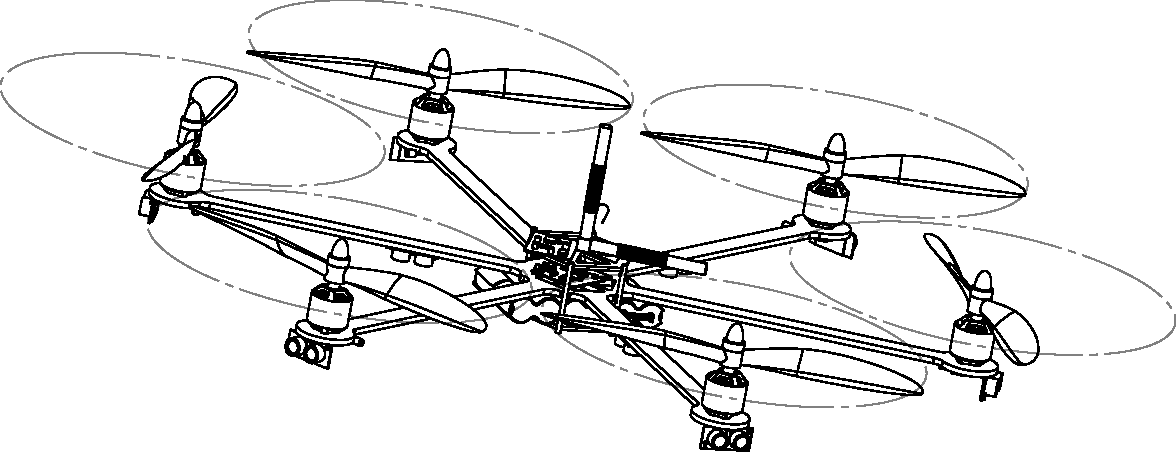
\includegraphics[scale=0.15]{../../img/hexacopterB.pdf}};
%	\coordinate [at=(hexacopter),yshift=-10] (hexapin);
%	\draw (hexapin) -- node[pos=1,ellipse,draw=black, minimum width=120, minimum height=70,rotate=0,dashed,xslant=1,fill=gray,opacity=0.4] {} ++(0,-1.5) coordinate(circlecenter);
%	\node at (circlecenter) [circle,fill=black,inner sep=1pt] {};
% 	\node [at=(nodo_1_3), yshift=7.5,xshift=7.5] {$\mathbf{p}_0$};
%	\node [at=(nodo_3_1), yshift=7.5,xshift=7.5] {$\mathbf{p}_n$};
%	\coordinate [at=(nodo_1_3),xshift=-60] (direction1); \coordinate [at=(nodo_1_1),xshift=-60] (direction2);
%	\draw [->,line width=2] (direction1) -- node[pos=0.5,above,rotate=45]{Plane direction} (direction2);
%	\coordinate [at=(circlecenter),shift=(150:1.3)] (labelA);
%	\draw [<-](labelA) -- ++(150:1) -- ++(-2,0) node[above,pos=0.5]{\scriptsize{Receiver range}};
%
%\end{tikzpicture}

% \begin{tikzpicture}[auto,node distance=10mm and 7mm, >=latex']

% 	\node [block, fill=gray!40] (hexamodel) {Hexacopter Model};
% 	\fromworkspace{parameter}{\scriptsize{Parameters}}{at=(hexamodel),xshift=-50,yshift=30}
% 	\node [sum, left=of hexamodel] (sumA) {$+$};
% 	\node [block, left=of sumA] (force) {$F_i = \dfrac{mg}{6}$};
	
% 	\node [ellipse, draw, minimum width=1.3cm, above=of force] {\scriptsize{Time}};
% 	\node [block,below=of hexamodel] (controller) {LQR Controller};
% 	\node [block, right=of controller] (integrator) {$\dfrac{1}{s}$};
% 	\fromworkspace{zattitude}{\scriptsize{$\hat{\mathbf{z}}$ attitude}}{at=(controller),yshift=-30,xshift=-50}
% 	\node [sum, right=of integrator] (sumB) {$+$};
% 	\node [block, right=of sumB, text width=2cm,align=center] (searching) {Searching Algorithm};
% 	\node [block, below=of searching, text width=2cm,align=center] (obstacle) {Obstacle Avoiding};
% 	\coordinate[at=(hexamodel),xshift=220] (intersection);
% 	\toworkspace{results}{$\mathbf{x}$}{right=of intersection};

% 	\draw [->] (force) -- (sumA);
% 	\draw [->] (sumA) -- (hexamodel);
% 	\draw [->] (hexamodel) -- (results_in);
% 	\draw [->] (searching) -- (sumB);
% 	\draw [->] (sumB) -- (integrator);
% 	\draw [->] (integrator) -- (controller);

% 	\draw [->] (controller) -| (sumA);
% 	\draw [->] (zattitude_out) -| (controller);
% 	\draw [->] (parameter_out) -| (hexamodel);
% 	\draw [->] (obstacle) -| (sumB);
% 	\draw [->] (intersection) |- (searching);
% 	\draw [->] (intersection) |- (obstacle);

% \end{tikzpicture}

% \salta

% \begin{tikzpicture}[auto,node distance=10mm and 7mm, >=latex]
% 	\inputpin{stato}{$\mathbf{x}$}{}
% 	\draw [at=(stato), xshift=50, fill=black] ++(0,0) node(muxin){} -- ++(0,2cm) -- ++(1mm,0) -- node[pos=0.2](posizione){} node[pos=0.4](velocita){} node[pos=0.6](angolo){} node[pos=0.8](velrotazione){} ++(0,-4cm) -- ++(-1mm,0) -- cycle;
% 	\node [sum, at=(posizione), xshift=50] (sumA) {$+$};
% 	\node [sum, at=(angolo), xshift=100] (sumB) {$+$};
% 	\draw [at=(stato), xshift=200+1mm, fill=black] ++(0,0) node(muxout){} -- ++(0,2cm) -- ++(-1mm,0) -- node[pos=0.2](posizioneB){} node[pos=0.4](velocitaB){} node[pos=0.6](angoloB){} node[pos=0.8](velrotazioneB){} ++(0,-4cm) -- ++(1mm,0) -- cycle;
% 	\node [gain,at=(stato.west), xshift=255, regular polygon rotate=-90] (gain) {$K$};
% 	\outputpin{controllo}{$\mathbf{u}$}{at=(stato.west), xshift=315};

% 	\inputpin{refer}{$\mathbf{x}_f$}{at=(stato.center), yshift=-80}
% 	\inputpin{attitz}{$\psi_f$}{at=(stato.center), yshift=-110}

% 	\draw [->] (stato_out) -- (muxin.center);
% 	\draw [->] (posizione.west) -- node[text width=1.5cm,align=left,pos=0.60]{\scriptsize{Position}} (sumA.west);
% 	\draw [->] (sumA.east) -- (posizioneB.west);
% 	\draw [->] (velocita.west) -- node[text width=1.5cm,align=left,pos=0.175]{\scriptsize{Velocity}} (velocitaB.west);
% 	\draw [->] (angolo.west) -- node[text width=1.5cm,align=left,pos=0.275]{\scriptsize{Attitude}} (sumB.west);
% 	\draw [->] (sumB.east) -- (angoloB.west);
% 	\draw [->] (velrotazione.west) -- node[text width=1.5cm,align=left,pos=0.175]{\scriptsize{Ang.ratio}} (velrotazioneB.west);
% 	\draw [->] (muxout.center) -- (gain);
% 	\draw [->] (gain) -- (controllo_in);

% 	\draw [->,draw=white,line width=2] (refer_out) -| (sumA.south);
% 	\draw [->,draw=white,line width=2] (attitz_out) -| (sumB.south);
% 	\draw [->] (refer_out) -| node[right,at end]{$-$} (sumA.south);
% 	\draw [->] (attitz_out) -| node[right,at end]{$-$} (sumB.south);

% \end{tikzpicture}

% \salta

% \begin{tikzpicture}[auto,node distance=10mm and 10mm, >=latex]
	
% 	\inputpin{stato}{$\mathbf{x}$}{}
% 	\node [block, right=of stato_out,fill=gray!40] (Hfield) {$\mathbf{H}\left( \mathbf{x}, \mathbf{p}_T, \hat{\mathbf{m}} \right)$};
% 	\fromworkspace{mvector}{\scriptsize{Magnetic Dipole $\hat{\mathbf{m}}$}}{at=(Hfield),xshift=-60,yshift=30,text width=2.7cm}
% 	\fromworkspace{tpos}{\scriptsize{Transmitter position $\mathbf{p}_T$}}{at=(Hfield),xshift=-60,yshift=50,text width=2.7cm}

% 	\coordinate [right=of Hfield] (intersection);
% 	\node [block, below=of intersection,text width=1cm, align=center] (absolute) {$|\mathbf{H}|$};
% 	\node [sum, below=of absolute] (prod) {$\times$};
% 	\node [block, left=of prod] (noise) {$\mathcal{N}(\mathbf{0},\Sigma)$};
% 	\node [gain, right=of prod, regular polygon rotate=-90, text width=0.3cm] (gain) {\scriptsize{SNR}};
% 	\node [sum, at=(intersection), xshift=100] (somma) {$+$};
% 	\outputpin{hvalue}{$\mathbf{H}$}{right=of somma}

% 	\draw[->] (stato_out) -- (Hfield);
% 	\draw[->] (Hfield) -- (somma);
% 	\draw[->] (somma) -- (hvalue_in);
% 	\draw[->] (intersection) -- (absolute);
% 	\draw[->] (absolute) -- (prod);
% 	\draw[->] (noise) -- (prod);
% 	\draw[->] (prod) -- (gain);
% 	\draw[->] (gain) -| (somma);
% 	\draw[->] (mvector_out) -| (Hfield);
% 	\draw[->] (tpos_out) -| (Hfield);

% \end{tikzpicture}

% \salta

% \begin{tikzpicture}[auto,node distance=10mm and 7mm, >=latex]
% 	\inputpin{stato}{$\mathbf{x}$}{}
% 	\coordinate [right=of stato_out] (intersectionA);
% 	\node [block, right=of intersectionA] (Hfield) {$\mathbf{H}$ sensor};
% 	\fromworkspace{mvector}{\scriptsize{Magnetic Dipole $\hat{\mathbf{m}}$}}{at=(Hfield),xshift=-60,yshift=30,text width=2.7cm}
% 	\fromworkspace{tpos}{\scriptsize{Transmitter position $\mathbf{p}_T$}}{at=(Hfield),xshift=-60,yshift=50,text width=2.7cm}
% 	\coordinate [right=of Hfield] (intersectionB);
% 	\node [block, right=of intersectionB] (direction){$\begin{array}{l} |\mathbf{H}| \\ \cos(\theta) \\ \sin(\theta) \end{array}$};
% 	\node [block, right=of direction] (filtering) {$\dfrac{\alpha_1 s + 1}{\beta_1 s^2 + \beta_2 s +1}$};
% 	\node [block,right=of filtering,text width=2cm,align=center] (velocity) {Exploration direction};
% 	\outputpin{velout}{$\mathbf{v}$}{right=of velocity}
% 	\node [block,below=of filtering,fill=gray!40,text width=3cm,align=center, minimum height=2cm] (emulation) {Emulation ${(\mathbf{H} - \hat{\mathbf{H}})^2 = \mathbf{0}}$};
% 	\coordinate [at=(emulation.east), yshift=15] (emulation_out1);
% 	\coordinate [at=(emulation.east), yshift=-15] (emulation_out2);
% 	\coordinate [at=(emulation.west), yshift=15] (emulation_in1);
% 	\coordinate [at=(emulation.west), yshift=-15] (emulation_in2);

% 	\toworkspace{posopt}{Optimized $\mathbf{p}_T$}{right=of emulation_out1}
% 	\toworkspace{mopt}{Optimized $\hat{\mathbf{m}}$}{right=of emulation_out2}
% 	\fromworkspace{paramV}{\scriptsize{Parameters}}{at=(velocity),xshift=-45,yshift=30}

% 	\draw [->] (mvector_out) -| (Hfield);
% 	\draw [->] (tpos_out) -| (Hfield);
% 	\draw [->] (stato_out) -- (Hfield);
% 	\draw [->] (Hfield) -- (direction);
% 	\draw [->] (direction) -- (filtering);
% 	\draw [->] (filtering) -- (velocity);
% 	\draw [->] (velocity) -- (velout_in);
% 	\draw [->] (intersectionA) |- (emulation_in2);
% 	\draw [->] (intersectionB) |- (emulation_in1);
% 	\draw [->] (emulation_out1) -- (posopt_in);
% 	\draw [->] (emulation_out2) -- (mopt_in);
% 	\draw [->] (paramV_out) -| (velocity);
% \end{tikzpicture}

% \salta

% \begin{tikzpicture}[auto,node distance=10mm and 7mm, >=latex]
% 	\inputpin{stato}{$\mathbf{x}$}{}
% 	\coordinate [right=of stato_out] (intersectionA);
% 	\node [block, right=of intersectionA,fill=gray!40] (range_finder) {Range Finder Model ${d_i}$};
% 	\fromworkspace{punti}{\scriptsize{${\Psi = [\mathbf{x}_i:i=1..M]}$}}{at=(range_finder),xshift=-60,yshift=30,text width=2cm}
% 	\fromworkspace{parametri}{\scriptsize{$[h,\,\rho]$}}{at=(range_finder),xshift=-60,yshift=50,text width=2cm}
% 	\node [block, below=of range_finder] (rotmat) {${\mathcal{R}^T(\phi,\theta,\psi)}$};
% 	\node [block, right=of range_finder] (velocita) {${\mathbf{v}_b = \sum\limits_{i=1}^{6} v(d_i) \hat{\mathbf{u}}_i}$};
% 	\node [sum, right=of velocita] (prod) {$\times$};
% 	\outputpin{velout}{$\mathbf{v}$}{right=of prod}
% 	\fromworkspace{paramV}{\scriptsize{$[p_1,\,p_2,\,p_3]$}}{at=(velocita),xshift=-45,yshift=30}

% 	\draw [->] (stato_out) -- (range_finder);
% 	\draw [->] (range_finder) -- (velocita);
% 	\draw [->] (velocita) -- (prod);
% 	\draw [->] (prod) -- (velout_in);
% 	\draw [->] (intersectionA) |- (rotmat);
% 	\draw [->] (rotmat) -| (prod);
% 	\draw [->] (punti_out) -| (range_finder);
% 	\draw [->] (parametri_out) -| (range_finder);
% 	\draw [->] (paramV_out) -| (velocita);

% \end{tikzpicture}

%\begin{tikzpicture}[auto,>=latex']
%	\coordinate (center);
%	\coordinate[at=(center.0), anchor=mid, shift=(62.05-90:0.6mm)] (pointA1);
%	\coordinate[at=(center.0), anchor=mid, shift=(153.3-90:1mm)] (pointB1);
%	\coordinate[at=(center.0), anchor=mid, shift=(260-90:1mm)] (pointC1);
%	
%	\coordinate[at=(pointA1.0), anchor=mid, shift=(0-90:15mm)] (pointA2);
%	\coordinate[at=(pointB1.0), anchor=mid, shift=(124.1-90:14.5mm)] (pointB2);
%	\coordinate[at=(pointC1.0), anchor=mid, shift=(180-90:15.5mm)] (pointC2);
%
%	\filldraw[fill=gray, draw=black] (pointA1) -- (pointA2) arc (0-90:124.1-90:15mm) -- cycle;
%	\filldraw[fill=white, draw=black] (pointB1) -- (pointB2) arc (124.1-90:180-91.5:15mm) -- cycle;
%	\filldraw[fill=gray, draw=black] (pointC1) -- (pointC2) arc (180-90:360-90:15.5mm) -- cycle;
%
%	\node[at=(pointA1.0), anchor=(0), shift=(-15:13mm)] {34\%};
%	\node[at=(pointB1.0), anchor=(0), shift=(40:13mm)] {16\%};
%	\node[at=(pointC1.0), anchor=(0), shift=(180:3mm)] {50\%};
%
%	\node[at=(pointA1.0), anchor=(180), shift=(-80:20mm), text width=2cm] {\scriptsize{2 or 3 buried person}};
%	\node[at=(pointB1.0), anchor=(180), shift=(80:20mm), text width=2cm] {\scriptsize{more than 3 buried person}};
%	\node[at=(pointC1.0), anchor=(180), shift=(140:29mm), text width=2cm] {\scriptsize{1 buried person}};
%
%\end{tikzpicture}
%
%\vspace{3cm}
%\begin{tikzpicture}[auto,node distance=1cm,>=latex']
%
%	\node[regular polygon, regular polygon sides=3, regular polygon rotate=180, draw, minimum height=1cm] (ant) {};
%	\draw (ant.north) -- (ant.south);
%	
%	\node[below of=ant] (input) {};
%\begin{scope}[node distance=4mm and 6mm]
%	\node[block, right=of input, minimum width=2.3cm, text width=2cm, align=center] (b1) {\scriptsize{Triple Antennas}};
%	\node[block, right=of b1, minimum width=2.3cm, text width=2cm, align=center] (b2) {\scriptsize{Frequency shift \\ Anti--alias filter}};
%	\node[block, below=of b2, minimum width=2.3cm, text width=2cm, align=center] (b3) {\scriptsize{A--D \\ Conversion}};
%	\node[block, below=of b3, fill=white, minimum width=2.3cm, text width=2cm, align=center] (b4) {\scriptsize{Digital Filter}};
%	\node[block, left=of b4, minimum width=2.3cm, text width=2cm, align=center] (b5) {\scriptsize{Signal \\ Detection}};
%	\node[block, left=of b5, minimum width=2.3cm, text width=2cm, align=center] (b6) {\scriptsize{H--field \\ Estimation}};
%\end{scope}
%
%	\draw[->] (ant.south) |- (b1) {};
%	\draw[->] (b1) -- (b2) {};
%	\draw[->] (b2) -- (b3) {};
%	\draw[->] (b3) -- (b4) {};
%	\draw[->] (b4) -- (b5) {};
%	\draw[->] (b5) -- (b6) {};
%	\node [at=(b3.0), anchor=(180), shift=(0:3mm)] (n1) {};
%	\node [at=(b3.0), anchor=(180), shift=(180:88mm)] (n2) {};
%	\draw [dashed] (n2) -- (b3) {};
%	\draw [dashed] (n1) -- (b3) {};
%
%	\node [at=(n2.0), anchor=(180), shift=(25:10mm)] (n1) {Analog};
%	\node [at=(n2.0), anchor=(180), shift=(-25:10mm)] (n1) {Digital};	
%\end{tikzpicture}
%
%\vspace{3cm}
%\begin{tikzpicture}[auto, node distance=2cm,>=latex']
%
%	\matrix [draw=white, row sep=0.1cm, column sep=1.5cm] {	
%	   	& \node [block, right, anchor=west, text width=1.5cm, minimum width=1.5cm] (levelD) {Level 3}; & \\
%		& \node [block, right,anchor=west, text width=1.8cm, minimum width=1.8cm] (levelC) {Level 2}; & \\
%	 	& \node [block, right,anchor=west, text width=2.1cm, minimum width=2.1cm] (levelB) {Level 1}; & \\
%		\node [input,right] (input) {}; & \node [block,anchor=west, text width=2.4cm, right, minimum width=2.4cm] (levelA) {Level 0}; & \node[output](output){} ; \\
% 	};
%
%	\draw [->] (input) -- node[below](mid) {Sensors} (levelA);
%	\draw [->] (mid) |- node {} (levelB);
%	\draw [->] (mid) |- node(midU) {} (levelC);
%	\draw [->] (mid) |- node (midUb)  {} (levelD);
%	\draw [->] (levelA) -- node[below] (midA) {Actuators} (output);
%	\draw [->] (levelB) -| node[pos=0.3] (midB) {} (midA);
%	\draw [->] (levelC) -| node[pos=0.3] (midC) {} (midB.south);
%	\draw [->] (levelD) -| node[pos=0.3] (midD) {} (midC.south);
%
%	\draw [->,dotted] (midUb.south) -- node  {} ++(0,0.8);
%	\draw [<-,dotted] (midD.south) -- node {} ++(0,0.8);
%\end{tikzpicture}
%\vspace{2cm}
%
%
%\begin{tikzpicture}[auto, node distance=2cm,>=latex']
%	\node[input] (input) {};
%	\node[block,right of=input] (perception) {Perception};
%	\node[block,right of=perception] (action) {Action};
%	\node[output, right of=action] (output) {};
%
%	\draw[->] (input) -- node[pos=0.2] {Sensors} (perception);
%	\draw[->] (perception) -- (action);
%	\draw[->] (action) -- node[pos=0.7] {Actuators} (output);
%\end{tikzpicture}
%
%\vspace{2cm}
%
%
%\begin{tikzpicture}[auto, node distance=1cm,>=latex']
%	\node [rectangle, draw=black, minimum width=6cm,minimum height=4.5cm] (envir) {};
%	\node [rectangle, draw=black, minimum width=4cm,minimum height=3.5cm] (body) at ++(0.75cm,-0.25cm) {};
%	\node [rectangle, draw=black, dashed, minimum width=2cm,minimum height=2cm] (body) at ++(1.5cm,-0.75cm) {};
%	\node [rectangle, fill=white] (situatedness) at ++(-1.25cm,-0.5cm) {$\underset{situatedness}{\longleftrightarrow}$};
%	\node [rectangle, fill=white] (embodiment) at ++(.5cm,-1.25cm) {$\underset{embodiment}{\longleftrightarrow}$};
%	\node [rectangle, fill=white, draw=black] at ++(-1.5cm,2.3cm) {\textbf{Environment}};
%	\node [rectangle, fill=white, draw=black] at ++(1.8cm,1.5cm) {\textbf{Agent}};
%	\node at(-0.6cm,1.1cm) {Body};
%	\node at(1.1cm,-0.1cm) {Mind};
%\end{tikzpicture}
%
%
%
%\vspace{2cm}
%\begin{tikzpicture}[auto, node distance=2.7cm,>=latex']
%	% EMULATION
%	\matrix[draw=black, row sep=0.1cm, column sep=0.2cm] (emulator) {
%	 \node {\scriptsize{Model}}; \\ 
%	 \node {\scriptsize{Hypothesis}};  \\
%	};
%	\node[above of=emulator] at ++(0,-1.8cm) {Emulator};
%
%	% GROUNDING
%	\matrix [draw=black,minimum width=4cm, minimum height=2.5cm, row sep=0.1cm, column sep=1cm, above of=emulator] (grounding) at ++(0,0cm) {	
%		& \node [block, right,anchor=west, minimum width=1cm ,minimum height=0.5cm] (levelC) {}; & \\
%	 	& \node [block, right,anchor=west, minimum width=1.25cm ,minimum height=0.5cm] (levelB) {}; & \\
%		\node [input,right] (input) {}; & \node [block,anchor=west, right, minimum width=1.5cm, minimum height=0.5cm] (levelA) {}; & \node[output](output){} ; \\
% 	};
%	\node[above of=grounding] at ++(0,1.5cm) {Grounding};
%
%	% EMULATOR
%	\node[block,below of=emulator] (environment) at ++(0,1.2cm) {\textbf{Environment}};
%
%
%	\draw [->] (input) -- node[below](mid) {} (levelA);
%	\draw [->] (mid) |- node (midK) {} (levelB);
%	\draw [->] (mid) |- node(midU) {} (levelC);
%	
%	\draw [->] (levelA) -- node[below] (midA) {} (output);
%	\draw [->] (levelB) -| node[pos=0.3] (midB) {} (midA);
%	\draw [->] (levelC) -| node[pos=0.3] (midC) {} (midB.south);
%
%
%	\draw [->,dotted] (mid) -- node  {} ++(0,1.8);
%	\draw [<-,dotted] (midC.south) -- node {} ++(0,0.5);
%
%	\node[right of=grounding] (gr) {};
%	\node[left of=grounding] (gl) {};
%
%	\draw [->] (emulator.west) -|  (gl.south) |- (grounding);
%	\draw [<-] (emulator.east) -|  (gr.south) |- (grounding);
%
%	\node[block,minimum width=6cm, minimum height=5.25cm,dashed] (agent) at ++(0,1.9cm) {};
%	\node[above of=agent] at ++(0,2cm) {\textbf{Agent}};
%
%	\draw [<-] (environment.east) -- ++(2cm,0) |- (grounding);
%	\draw [<-] (environment.west) -- ++(-2cm,0) |- (grounding);
%
%\end{tikzpicture}

% \vspace{3cm}
% \begin{tikzpicture}[auto,node distance=0.5cm and 1cm, >=latex', minimum width=3cm, minimum height=1cm, text width=4cm, align=center]

% 	%\draw (0,0) ellipse (2cm and 1cm) node (start) {Start};
% 	%\draw

% 	\node [ellipse, draw, minimum width=2cm, text width=2cm, fill=gray!40] (start) {Start};
% 	\node [trapezium, draw, trapezium left angle=70,trapezium right angle=-70, below=of start] (inserimento) {Receiving starting point $\mathbf{p}_0$, ending point $\mathbf{p}_n$, plane direction};
% 	\node [rectangle, draw, below=of inserimento] (generazione_punti) {Generation of points vector $\mathbf{P} = [\mathbf{p}_0,\dots,\mathbf{p}_n]$, set confidence distance $\Delta$};
% 	\node [rectangle, draw, below=of generazione_punti] (abilita_ricerca) {Start searching sensors, start radar detection routines $\Lambda(\mathbf{s}) \overset{?}{<>} \eta$ };
% 	\node [rectangle, draw, below=of abilita_ricerca] (goto_start) {$i \leftarrow 0$};
% 	\node [rectangle, draw, below=of goto_start, text width=2cm] (select_point) {Go To $\textbf{p}_i$};
% 	\node [trapezium, draw, trapezium left angle=70, trapezium right angle=-70, below=of select_point,text width=1.2cm] (read_position) {Get $\mathbf{x}$};
% 	\node [diamond, draw, aspect=2, text width=2.3cm, below=of read_position] (distanza) {$\left| \mathbf{p}_i - \mathbf{x} \right| < \Delta$ ?};
% 	\node [diamond, draw, aspect=2, text width=2cm, below=of distanza] (lastpoint) {$i = n$ ?};
% 	\node [ellipse, draw, minimum width=2cm, text width=2cm, below=of lastpoint,fill=gray!40] (stop) {Stop};

% 	\node [rectangle,draw,left=of lastpoint, text width=1.5cm] (addone) { $i \leftarrow i+1$ };
% 	\coordinate [at=(select_point.north), shift=(0:22mm)] (braces_a);
% 	\coordinate [at=(distanza.south), shift=(0:22mm)] (braces_b);
% 	\draw [decorate,decoration={brace,amplitude=12pt}] (braces_a) -- (braces_b) {};

% 	\node [diamond, draw, aspect=2, text width=2cm, at=(read_position.north east), shift=(0:50mm)] (detection) {$\Lambda(\mathbf{s}) > \eta$?};
% 	\node [rectangle, draw,fill=gray!40, text width=2.5cm, below=of detection] (search) {Search \mbox{H--field} source};

% 	\coordinate [at=(detection.north), shift=(90:5mm)] (extraA);
% 	\coordinate [at=(search.south), shift=(270:5mm)] (extraB);
% 	\coordinate [at=(detection.west), shift=(180:5mm)] (extraC);
% 	\coordinate [at=(distanza.west), shift=(180:10mm)] (intraB);

% 	\draw [->] (start) -- (inserimento);
% 	\draw [->] (inserimento) -- (generazione_punti);
% 	\draw [->] (generazione_punti) -- (abilita_ricerca);
% 	\draw [->] (abilita_ricerca) -- (goto_start);
% 	\draw [->] (goto_start) -- coordinate[pos=0.5](intraA) (select_point);
% 	\draw [->] (select_point) -- (read_position);
% 	\draw [->] (read_position) -- (distanza);
% 	\draw [->] (distanza) -- node[shift=(0:-17mm)]{\scriptsize{true}} (lastpoint);
% 	\draw [->] (lastpoint) -- node[shift=(0:-17mm)]{\scriptsize{true}} (stop);
% 	\draw [->] (detection) -- node[shift=(0:-17mm)]{\scriptsize{true}} (search);
% 	\draw [->] (lastpoint) -- node[shift=(45:3mm)]{\scriptsize{false}} (addone);

% 	\draw [->,dashed] (extraA) -- (detection);
% 	\draw [->,dashed] (search) -- (extraB);
% 	\draw [->,dashed] (detection) -- node[shift=(45:3mm)]{\scriptsize{false}} (extraC);

% 	\draw [->] (addone) |- (intraA);
% 	\draw (distanza) -- node[shift=(45:3mm)]{\scriptsize{false}} (intraB) |- (intraA);

% \end{tikzpicture}

% \newcommand{\drawcube}[9]{%
% 	\coordinate (#7_A) at (#1,#2,#3);%
% 	\coordinate (#7_B) at (#1+#4,#2,#3);%
% 	\coordinate (#7_C) at (#1+#4,#2+#5,#3);%
% 	\coordinate (#7_D) at (#1,#2+#5,#3);%
% 	\coordinate (#7_E) at (#1+#4,#2,0);%
% 	\coordinate (#7_F) at (#1+#4,#2+#5,0);%
% 	\coordinate (#7_G) at (#1,#2+#5,0);%
% 	%
% 	\filldraw [draw=black, fill=#6] (#7_A) -- (#7_B) -- (#7_C) -- (#7_D) -- cycle;%
% 	\filldraw [draw=black, fill=#6] (#7_B) -- (#7_C) -- (#7_F) -- (#7_E) -- cycle;%
% 	\filldraw [draw=black, fill=#6] (#7_D) -- (#7_C) -- (#7_F) -- (#7_G) -- cycle;%
% 	\node [#9] at (0.5*#4+#1,0.5*#5+#2,#3) {#8};%
% }

% \newcommand{\drawplanezy}[8]{%
% 	\coordinate (#5_A) at (#1,#2,#3);%
% 	\coordinate (#5_B) at (#1,#2,0);%
% 	\coordinate (#5_C) at (#1,#2+#4,0);%
% 	\coordinate (#5_D) at (#1,#2+#4,#3);%
% 	\draw [#6] (#5_A) -- (#5_B) -- (#5_C) -- (#5_D) -- cycle;%
% 	\node [#8] at (#1,#2+#4-0.4,0.5*#3) {#7};%
% }

% \newcommand{\drawplanexy}[7]{%
% 	\coordinate (#7_A) at (#1,#2,#3);%
% 	\coordinate (#7_B) at (#1+#4,#2,#3);%
% 	\coordinate (#7_C) at (#1+#4,#2+#5,#3);%
% 	\coordinate (#7_D) at (#1,#2+#5,#3);%
% 	\draw [#6] (#7_A) -- (#7_B) -- (#7_C) -- (#7_D) -- cycle;%
% }


% \begin{tikzpicture}[>=latex']
% 	\drawplanexy{-0.3}{-0.3}{-0.3}{6.7}{10}{dashed}{perception}
% 	\node [at=(perception_D),xshift=30,yshift=-10] {\textbf{Perception}};
% 	\drawcube{0}{0}{5}{6.4}{1}{white}{dinamica}{Dynamics and control}{};
% 	\drawcube{0}{1.2}{5}{6.4}{1}{white}{tracking}{Tracking Problem}{};
	
% 	\drawcube{0}{2.4}{5}{6.4}{1}{white}{ostacoli}{Obstacle Avoidance}{};
% 	\drawcube{0}{3.6}{5}{6.4}{1}{white}{altitude}{Altitude Keeping}{};
	
% 	\drawcube{0}{4.8}{5}{3}{1.5}{white}{source}{Source searching}{text width=2cm,align=center};
% 	\drawcube{0}{6.5}{5}{3}{1.5}{white}{emulatore}{Emulation}{text width=2cm,align=center};

% 	\drawplanezy{3.2}{4.8}{5}{4.5}{radar_det}{fill=white,opacity=0.90}{Radar detect}{rotate=45,xslant=1};

% 	\drawcube{3.4}{4.8}{5}{3}{3.2}{white}{alpha}{Exploration routines}{text width=2cm,align=center};
% 	\drawplanexy{-0.3}{-0.3}{5.3}{6.7}{10}{dashed}{action}
% 	\node [at=(action_D),xshift=20,yshift=-10] {\textbf{Action}};

% 	\draw [->,line width=1.5] (action_D) -- ++(0,0,2);
% 	\draw [->,line width=1.5] (perception_D) -- ++(0,0,2);

% 	\coordinate [at=(radar_det_D), yshift=-20] (arrows_point);
% 	\draw [->,dashed]  (arrows_point) -- ++(1.5,0,0); 
% 	\draw [->,dashed]  (arrows_point) -- ++(-1.5,0,0); 
% \end{tikzpicture}

% \vspace{2cm}

% \begin{tikzpicture}[>=latex',scale=0.4]
% 	\drawplanexy{-0.3}{-0.3}{-0.3}{6.7}{10}{dashed}{perception}
	
% 	\drawcube{0}{0}{5}{6.4}{1}{white}{dinamica}{}{};
% 	\drawcube{0}{1.2}{5}{6.4}{1}{white}{tracking}{}{};
	
% 	\drawcube{0}{2.4}{5}{6.4}{1}{white}{ostacoli}{}{};
% 	\drawcube{0}{3.6}{5}{6.4}{1}{white}{altitude}{}{};
	
% 	\drawcube{0}{4.8}{5}{3}{1.5}{white}{source}{}{};
% 	\drawcube{0}{6.5}{5}{3}{1.5}{white}{emulatore}{}{};

% 	\drawplanezy{3.2}{4.8}{5}{4.5}{radar_det}{fill=white,opacity=0.90}{}{};

% 	\drawcube{3.4}{4.8}{5}{3}{3.2}{white}{alpha}{}{};
% 	\drawplanexy{-0.3}{-0.3}{5.3}{6.7}{10}{dashed}{action}
	

% 	\draw [->,line width=1.5] (action_D) -- ++(0,0,2);
% 	\draw [->,line width=1.5] (perception_D) -- ++(0,0,2);

% 	\coordinate [at=(radar_det_D), yshift=-5] (arrows_point);
% 	\draw [->,dashed]  (arrows_point) -- ++(1.5,0,0); 
% 	\draw [->,dashed]  (arrows_point) -- ++(-1.5,0,0); 
% \end{tikzpicture}

\end{document}